%!TEX root = ../lectures.tex

\topic{Trigonometric Derivatives, continued}

Recall from last time how
\[
	\lim_{x \to 0} \frac{\sin(x)}{x} = 1.
\]

\noindent
Using this we can prove

\begin{proposition}
	$\displaystyle \frac{d}{d x} \sin(x) = \cos(x)$.
\end{proposition}

\begin{proof}
	We need the identity $\sin(\alpha + \beta) = \sin(\alpha) \cos(\beta) + \cos(\alpha) \sin(\beta)$.
	Then
	\begin{align*}
		\frac{d}{d x} \sin(x) & = \lim_{h \to 0} \frac{\sin(x + h) - \sin(x)}{h}                                                                                                                                             \\
		                      & = \lim_{h \to 0} \frac{\sin(x) \cos(h) + \cos(x) \sin(h) - \sin(x)}{h}                                                                                                                       \\
		                      & = \lim_{h \to 0} \frac{\sin(x) (\cos(h) - 1) + \cos(x) \sin(h)}{h}                                                                                                                           \\
		                      & = \Big ( \lim_{h \to 0} \sin(x) \Big ) \cdot \Big ( \lim_{h \to 0} \frac{\cos(h) - 1)}{h} \Big ) + \Big ( \lim_{h \to 0} \cos(x) \Big ) \cdot \Big ( \lim_{h \to 0} \frac{\sin(h)}{h} \Big ) \\
		                      & = \sin(x) \cdot 0 + \cos(x) \cdot 1 = \cos(x).
	\end{align*}

	\noindent
	The only mystery in the above computation is the $\cos(h)$ limit in the penultimate line.
	We shed light on it by using $\cos(h) = 1 - 2 (\sin(h / 2))^2$, like so
	\[
		\lim_{h \to 0} \frac{\cos(h) - 1}{h} = - \lim_{h \to 0} \frac{2 (\sin(h / 2))^2}{h},
	\]
	which if we let $x = h / 2$ (which also approaches $0$ as $h$ does) becomes
	\[
		- \lim_{x \to 0} \frac{\sin(x)}{x} \cdot \sin(x) = -1 \cdot 0 = 0. \qedhere
	\]
\end{proof}

\noindent
Since we have a chain rule, it is immediate to find the derivative of $\cos$ once we know the derivative of $\sin$.

\begin{corollary}
	$\displaystyle \frac{d}{d x} \cos(x) = - \sin(x)$.
\end{corollary}

\begin{proof}
	We know that $\cos(x) = \sin(\pi/2 - x)$, and $\sin(x) = \cos(\pi/2 - x)$, whence by the chain rule
	\begin{align*}
		\frac{d}{d x} \cos(x) & = \frac{d}{d x} \sin\Big ( \frac{\pi}{2} - x \Big ) = \cos \Big ( \frac{\pi}{2} - x \Big ) \cdot \frac{d}{d x} \Big ( \frac{\pi}{2} - x \Big ) \\
		                      & = - \cos \Big ( \frac{\pi}{2} - x \Big ) = - \sin(x). \qedhere
	\end{align*}
\end{proof}

\begin{exercise}
	Use the computational rules to find the derivatives of $\tan$, $\sec$, $\cot$, and $\csc$, in the event that you like these functions.
\end{exercise}

\noindent
Since so far the discussion about derivatives has been quite heavy on theory, we close it off with a number of computational problems, so as to hopefully get some practice with how the definition of the derivative works. In the future we will often end up computing derivatives directly using results such as these, instead of falling back on the definition in terms of the limit of a difference quotient.

\begin{exercises}
Show the following:
\begin{alphalist}
	\item $\displaystyle \frac{d}{d x} c = 0$, where $c$ is constant.
	\item $\displaystyle \frac{d}{d x} k x = k$, where $k$ is constant.
	\item $\displaystyle \frac{d}{d x} \frac{1}{x} = - \frac{1}{x^2}$.
	\item $\displaystyle \frac{d}{d x} \sqrt{x} = \frac{1}{2 \sqrt{x}}$.
	\item $\displaystyle \frac{d}{d x} x^n = n x^{n - 1}$, for all $n \in \Z$, perhaps using induction.
\end{alphalist}
\end{exercises}

\noindent
Note how, for instance, \fakeitemref{a}, \fakeitemref{b}, and \fakeitemref{e} combined, together with our computational rules, tell us how to differentiate every possible polynomial.

The majority of this lecture will be about the Mean-value theorem and some consequences thereof, but first we will wrap up the discussion of the derivative itself somewhat.

\topic{Higher Order Derivatives}

Since, by definition, the derivative of a function $y = f(x)$ is again a function, it can happen that the derivative itself is differentiable (at some point(s)).

We call this derivative of a derivative the \keyword{second derivative}\index{derivative!higher order}\index{derivative!second} of the original function.
Like the first derivative, there are many notations used for this:
\[
	y'' = f'' = \frac{d^2 y}{d x^2} = \frac{d}{d x} \frac{d}{d x} f = \frac{d^2}{d x^2} f = D_x^2 y = D_x^2 f.
\]

\noindent
We can continue this to achieve a general $n$th order derivative,
\[
	y^{(n)} = f^{(n)} = \frac{d^n y}{d x^n} = \frac{d^n}{d x^n} f = D_x^n y = D_x^n f,
\]
defined inductively as the derivative of the $(n - 1)$st order derivative.

\begin{remark}
	We use $y^{(n)}$ or $f^{(n)}$, with the parentheses, in order to distinguish higher order derivatives from exponents or compositions,
	\[
		y^n = \underbrace{y \cdot y \cdot \ldots \cdot y}_{n ~\text{lots of}~ y}, \qquad \text{or} \qquad  f^n = \underbrace{f \circ f \circ \cdots \circ f}_{n~\text{lots of}~f}.
	\]
\end{remark}

\noindent
For convenience the function itself is usually taken to be its own zeroth derivative, $f = f^{(0)}$.

\begin{example}
	The classical example is the reason calculus was invented: take $x = x(t)$ to be the position (of something) at the time $t$.
	Then its velocity is $v = \frac{d x}{d t} = x'$, and its acceleration is $a = \frac{d v}{d t} = \frac{d^2 x}{d t^2} = x''$.
	This exemplifies why we often want to think of the derivative as the rate of change of something.
\end{example}

\noindent
These higher order derivatives are often very important in physics, since it turns out that much in the real world can be modeled using so-called differential equations, which we will deal more with toward the end of the course.
For now, we'll discuss it briefly in an example.

\begin{example}
	Show that $y(t) = A \cos(k t) + B \sin(k t)$, for $A$, $B$, and $k$ constants, is a solution to the \keyword{second-order differential equation}\index{differential equation}\index{differential equation!second order}
	\[
		\frac{d^2 y}{d t^2} (t) + k^2 y(t) = 0.
	\]
	To do this we compute the second derivative and test it in the equation (when we deal with differential equations more thoroughly in the future we will learn how to find these solutions on our own):
	\[
		\frac{d^2 y}{d t^2}(t) = \frac{d}{d t} (-A k \sin(k t) + B k \cos(k t)) = -A k^2 \cos(k t) - B k^2 \sin(k t).
	\]
	We then insert it into the differential equation,
	\[
		\frac{d^2 y}{d t^2} (t) + k^2 y(t) = - k^2 (A \cos(k t) + B \sin(k t)) + k^2 (A \cos(k t) + B \sin(k t)) = 0
	\]
	for all $t$.
\end{example}

\topic{The Mean-Value Theorem}

\begin{example}
	Suppose we leave on a trip at 3 o'clock, traveling 100 kilometres away, and arriving 2 hours later, at 5 o'clock.
	Then of course our average speed was
	\[
		\frac{\SI{100}{\kilo\metre}}{\SI{2}{\hour}} = \SI[per-mode = symbol]{50}{\kilo\metre\per\hour}.
	\]
	We might not have traveled at this speed constantly (indeed it's unlikely we did, since we presumably started at rest and accelerated), but we \emph{must} have traveled at $\SI[per-mode = symbol]{50}{\kilo\metre\per\hour}$ at least once!

	If not, our speed was either always above or always below $\SI[per-mode = symbol]{50}{\kilo\metre\per\hour}$, in which case we would have arrived either before or after 5 o'clock.
\end{example}

\noindent
In the language of calculus, this is called the Mean-value theorem, and the crucial detail that makes it true is, of course, that our speed whilst traveling can't `jump'.
I.e., we can't go from $\SI[per-mode = symbol]{25}{\kilo\metre\per\hour}$ to $\SI[per-mode = symbol]{75}{\kilo\metre\per\hour}$ without ever passing $\SI[per-mode = symbol]{50}{\kilo\metre\per\hour}$.
Once again in the language of calculus, this is what we call continuity, and indeed since we have acceleration of some kind everywhere, even if constant, our speed (or velocity) must also have a derivative.

\begin{theorem}[Mean-value theorem]\index{mean-value theorem}
	Let $f$ be a function continuous on the closed and finite interval $[a, b]$ that is differentiable on $]{a, b}[$.
	Then there exists a point $c \in {]{a, b}[}$ such that
	\[
		\frac{f(b) - f(a)}{b - a} = f'(c).
	\]
\end{theorem}

\begin{figure}
	\centering
	\begin{tikzpicture}
		\begin{axis}[
			scale = 0.8,
			axis x line = left,
			axis y line = left,
			xmin = -1,
			xmax = 5,
			ymin = 0,
			ymax = 10,
			xlabel = $x$,
			ylabel = $y$,
			xtick = {0.5, 4.5},
			xticklabels = {$a$, $b$},
			ytick = {4.80134, 7.36554},
			yticklabels = {$f(a)$, $f(b)$},
			every axis x label/.style = {
				at = {(ticklabel* cs:1.01)},
				anchor = west,
			},
			every axis y label/.style = {
				at = {(ticklabel* cs:1.01)},
				anchor = south,
			},
			]
			\addplot[
			black,
			samples = 100,
			domain = 0.5:4.5,
			]{0.5*(x+2)*sin((2*(x+2))r)+6};
			\addplot[
			gray,
			dashed
			] coordinates {(0.5, 1.29134) (4.5, 3.85554)};
			\addplot[
			gray,
			dashed
			] coordinates {(0.5, 7.05234) (4.5, 9.61654)};
			\addplot[
			gray,
			dashed
			] coordinates {(0.5, 4.80134) (4.5, 7.36554)};
			\addplot[mark=*] coordinates {(0.5, 4.80134)};
			\addplot[mark=*] coordinates {(4.5, 7.36554)};
			\addplot[mark=*] coordinates {(1.90890, 7.95317)};
			\addplot[mark=*] coordinates {(3.59946, 3.25795)};
		\end{axis}
	\end{tikzpicture}
	\caption{Illustration of the Mean-value theorem.}
	\label{lec5:meanval}
\end{figure}


\noindent
That is to say, there must exist some point(s) in the interior of the interval with the same slope as the line segment connecting the two endpoints.

An example of this theorem is demonstrated in Figure \ref{lec5:meanval}, which also demonstrates that the $c$ in the theorem needn't be unique.
We will prove this in a bit, but for now we will establish some more theory and also motivate why both the continuity and the differentiability is required in Figure \ref{lec5:meanvalcounter}.

\begin{figure}
	\centering
	\begin{subfigure}{0.3\textwidth}
		\centering
		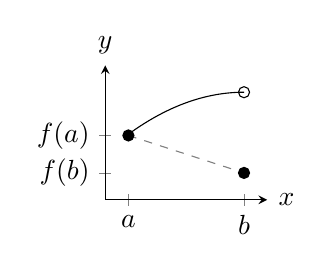
\begin{tikzpicture}
			\begin{axis}[
				scale = 0.3,
				axis x line = left,
				axis y line = left,
				xmin = 0,
				xmax = 3.5,
				ymin = 0,
				ymax = 10,
				xlabel = $x$,
				ylabel = $y$,
				xtick = {0.5, 3},
				xticklabels = {$a$, $b$},
				ytick = {4.785, 2},
				yticklabels = {$f(a)$, $f(b)$},
				every axis x label/.style = {
					at = {(ticklabel* cs:1.01)},
					anchor = west,
				},
				every axis y label/.style = {
					at = {(ticklabel* cs:1.01)},
					anchor = south,
				},
				]
				\addplot[
				black,
				samples = 100,
				domain = 0.5:3,
				]{-0.5*(x-3)^2+8};
				\addplot[
				gray,
				dashed
				] coordinates {(0.5, 4.785) (3, 2)};
				\addplot[mark=*] coordinates {(0.5, 4.785)};
				\addplot[mark=o] coordinates {(3, 8)};
				\addplot[mark=*] coordinates {(3, 2)};
			\end{axis}
		\end{tikzpicture}
		\caption{Discontinuous at endpoint}
	\end{subfigure}
	\quad
	\begin{subfigure}{0.3\textwidth}
		\centering
		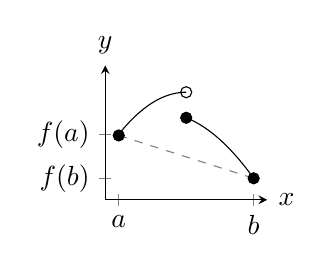
\begin{tikzpicture}
			\begin{axis}[
				scale = 0.3,
				axis x line = left,
				axis y line = left,
				xmin = 0,
				xmax = 6,
				ymin = 0,
				ymax = 10,
				xlabel = $x$,
				ylabel = $y$,
				xtick = {0.5, 5.5},
				xticklabels = {$a$, $b$},
				ytick = {4.875, 1.6},
				yticklabels = {$f(a)$, $f(b)$},
				every axis x label/.style = {
					at = {(ticklabel* cs:1.01)},
					anchor = west,
				},
				every axis y label/.style = {
					at = {(ticklabel* cs:1.01)},
					anchor = south,
				},
				]
				\addplot[
				black,
				samples = 100,
				domain = 0.5:3,
				]{-0.5*(x-3)^2+8};
				\addplot[
				black,
				samples = 100,
				domain = 3:5.5,
				]{-0.4*(x-2)^2+6.5};
				\addplot[
				gray,
				dashed
				] coordinates {(0.5, 4.785) (5.5, 1.6)};
				\addplot[mark=*] coordinates {(0.5, 4.785)};
				\addplot[mark=o] coordinates {(3, 8)};
				\addplot[mark=*] coordinates {(3, 6.1)};
				\addplot[mark=*] coordinates {(5.5, 1.6)};
			\end{axis}
		\end{tikzpicture}
		\caption{Discontinuous at interior point}
	\end{subfigure}
	\quad
	\begin{subfigure}{0.3\textwidth}
		\centering
		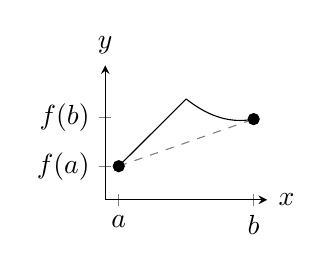
\begin{tikzpicture}
			\begin{axis}[
				scale = 0.3,
				axis x line = left,
				axis y line = left,
				xmin = 0,
				xmax = 6,
				ymin = 0,
				ymax = 10,
				xlabel = $x$,
				ylabel = $y$,
				xtick = {0.5, 5.5},
				xticklabels = {$a$, $b$},
				ytick = {2.5, 6.1},
				yticklabels = {$f(a)$, $f(b)$},
				every axis x label/.style = {
					at = {(ticklabel* cs:1.01)},
					anchor = west,
				},
				every axis y label/.style = {
					at = {(ticklabel* cs:1.01)},
					anchor = south,
				},
				]
				\addplot[
				black,
				samples = 100,
				domain = 0.5:3,
				]{2*x+1.5};
				\addplot[
				black,
				samples = 100,
				domain = 3:5.5,
				]{0.4*(x-5)^2+5.9};
				\addplot[
				gray,
				dashed
				] coordinates {(0.5, 2.5) (5.5, 6)};
				\addplot[mark=*] coordinates {(0.5, 2.5)};
				\addplot[mark=*] coordinates {(5.5, 6)};
			\end{axis}
		\end{tikzpicture}
		\caption{Not differentiable at interior point}
	\end{subfigure}
	\caption{Counterexamples of the Mean-value theorem where essential conditions are violated.}
	\label{lec5:meanvalcounter}
\end{figure}


This demonstrates that if we lack continuity anywhere in the closed interval, then we can construct a counter example, and likewise if we lack differentiability anywhere in the open interval, we may do the same.

We now prove an intermediary result we need in order to prove the Mean-value theorem.

\begin{lemma}\label{lec5:criticalpoint}
	If $f$ is defined on an open interval ${]{a, b}[}$ and achieves a maximum (or minimum) at $c \in {]{a, b}[}$, then if $f'(c)$ exists, it must be $0$.
\end{lemma}

\noindent
Such points where the derivative is $0$ are called \keyword{critical points}\index{critical point}.

\begin{proof}
	If $f$ has a maximum at $c \in {]{a, b}[}$, then $f(x) - f(c) \leq 0$ for all $x \in {]{a, b}[}$.
	We consider two cases:

	\fakeitem{1} If $c < x < b$, then
	\[
		\frac{f(x) - f(c)}{x - c} \leq 0,
	\]
	since $c < x$, which, if we recall the alternative difference quotient,\footnote{It is of course possible to compute the same with the $h \to 0$ type difference quotient, it's just marginally more cumbersome.} implies the sign of the right derivative at $c$,
	\[
		f'_+(c) = \lim_{x \to c} \frac{f(x) - f(c)}{x - c} \leq 0.
	\]

	\noindent
	\fakeitem{2} Similarly if $a < x < c$, then we have
	\[
		\frac{f(x) - f(c)}{x - c} \geq 0
	\]
	which similarly implies
	\[
		f'_-(c) = \lim_{x \to c} \frac{f(x) - f(c)}{x - c} \geq 0.
	\]

	\noindent
	By assumption $f'(c)$ exists, so it is equal to the left and right derivative at that point, so
	\[
		0 \leq f'_-(c) = f'(c) = f'_+(c) \leq 0,
	\]
	whereby $f'(c) = 0$.

	For the case of the minimum, the proof is almost identical, except we change the direction of certain inequalities.
\end{proof}

\noindent
We now show a special case of the Mean-value theorem, with which we later prove the full version.

\begin{theorem}[Rolle's theorem]\index{Rolle's theorem}
	Suppose that $f$ is a continuous function on the closed and finite interval $[a, b]$ and that it is differentiable on ${]{a, b}[}$.
	If $f(a) = f(b)$, then there exists a point $c \in {]{a, b}[}$ such that $f'(c) = 0$.
\end{theorem}

\begin{proof}
	There are two cases to consider.
	If $f(x) = f(a)$ for all $x \in [a, b]$, then $f$ is constant and $f'(c) = 0$ for all $c \in {]{a, b}[}$.

	Suppose that there exists some $x \in {]{a, b}[}$ such that $f(x) \neq f(a)$, so that either $f(x) > f(a)$ or $f(x) < f(a)$.

	Consider the $f(x) > f(a)$ case.
	Since $f$ is continuous on $[a, b]$, by the Max-min theorem $f$ must have a maximum at some point $c \in [a, b]$.
	Thus
	\[
		f(c) \geq f(x) > f(a) = f(b),
	\]
	so $c$ cannot be equal to $a$ or $b$, whereby $c \in {]{a, b}[}$, where by assumption $f$ is differentiable.
	Thus $f'(c)$ exists, and so by the previous lemma $f'(c) = 0$.

	For the $f(x) < f(a)$ case, we instead use the Max-min theorem to ensure the existence of a minimum, and proceed accordingly.
\end{proof}

\noindent
With this we are finally ready to prove the Mean-value theorem.

\begin{proof}[Proof of Mean-value theorem]
	Recall that $f$ is continuous on $[a, b]$ and differentiable on ${]{a, b}[}$.
	We define a new function $g$ by
	\[
		g(x) = f(x) - \Big ( f(a) + \frac{f(b) - f(a)}{b - a} \, (x - a) \Big ).
	\]
	The expression in the parentheses is the line segment joining $(a, f(a))$ and $(b, f(b))$, whereby $g(x)$ is the vertical distance between this line segment and $f$ itself at each point $x$, as illustrated in Figure \ref{lec5:meanvalproof}.
	\begin{figure}
		\centering
		\begin{tikzpicture}
			\begin{axis}[
				scale = 1,
				axis x line = left,
				axis y line = left,
				xmin = 0,
				xmax = 5,
				ymin = 0,
				ymax = 10,
				xlabel = $x$,
				ylabel = $y$,
				xtick = {0.5, 3, 4.5},
				xticklabels = {$a$, $c$, $b$},
				ytick = {2, 5.2},
				yticklabels = {$f(a)$, $f(b)$},
				every axis x label/.style = {
					at = {(ticklabel* cs:1.01)},
					anchor = west,
				},
				every axis y label/.style = {
					at = {(ticklabel* cs:1.01)},
					anchor = south,
				},
				]
				\addplot[
				gray,
				samples = 100,
				domain = 0.5:4.5,
				dashed
				]{-0.8*(x-3)^2+7};
				\addplot[
				gray,
				dashed
				] coordinates {(0.5, 2) (4.5, 5.2)};
				\addplot[
				black,
				solid,
				<->
				] coordinates {(3, 4.2) (3, 6.8)};
				\addplot[mark=*] coordinates {(0.5, 2)};
				\addplot[mark=*] coordinates {(4.5, 5.2)};
				\addplot[mark=*] coordinates {(3, 7)};
				\addplot[mark=*] coordinates {(3, 4)};
				\addplot[mark=none] coordinates {(2, 6.2)} node[pin=120:{$f(x)$}]{};
				\addplot[mark=none] coordinates {(3, 5.5)} node[pin=190:{$g(c)$}]{};
			\end{axis}
		\end{tikzpicture}
		\caption{The geometrical construction of $g$ in the proof of the Mean-value theorem.}
		\label{lec5:meanvalproof}
	\end{figure}

	Since $f$ is continuous on $[a, b]$ and differentiable on ${]{a, b}[}$, $g$ is as well.
	Moreover $g(a) = g(b) = 0$ (feel free to verify), whence by Rolle's theorem there exists a $c \in {]{a, b}[}$ such that $g'(c) = 0$.

	By differentiating $g$ we get
	\[
		g'(x) = f'(x) - \frac{f(b) - f(a)}{b - a},
	\]
	so at $x = c$ we have
	\[
		0 = f'(c) - \frac{f(b) - f(a)}{b - a} \qquad \Longleftrightarrow \qquad f'(c) = \frac{f(b) - f(a)}{b - a}.\qedhere
	\]
\end{proof}

\begin{corollary}[Generalised Mean-value theorem]
	If $f$ and $g$ are both continuous on $[a, b]$ and differentiable on ${]{a, b}[})$, and if $g'(x) \neq 0$ for all $x \in {]{a, b}[}$, then there exists a number $c \in {]{a, b}[}$ such that
	\[
		\frac{f(b) - f(a)}{g(b) - g(a)} = \frac{f'(c)}{g'(c)}.
	\]
\end{corollary}

\begin{proof}
	Note that $g(b) \neq g(a)$ since otherwise there would exist an $x \in {]{a, b}[}$ such that $g'(x) = 0$ by the Rolle's theorem.
	Thus the division in the left-hand side is well-defined.

	We apply the Mean-value theorem to
	\[
		h(x) = (f(b) - f(a))(g(x) - g(a)) - (g(b) - g(a)) (f(x) - g(a)).
	\]

	\noindent
	Since $h(a) = h(b) = 0$ (again, feel free to verify) and $h$ has the appropriate continuity and differentiability, there exists a $c \in {]{a, b}[}$ such that $h'(c) = 0$.
	Therefore
	\[
		h'(c) = (f(b) - f(a)) g'(c) - (g(b) - g(a)) f'(c) = 0
	\]
	which by rearranging becomes
	\[
		\frac{f(b) - f(a)}{g(b) - g(a)} = \frac{f'(c)}{g'(c)}. \qedhere
	\]
\end{proof}

\noindent
We end today's lecture with two nice consequences of the Mean-value theorem.

\begin{definition}[Increasing and decreasing functions]\label{lec5:monotonicity}
	Suppose $f$ is defined on some interval $I$ and that $x_1$ and $x_2$ are points on $I$.
	\begin{romanlist}
		\item If $f(x_2) > f(x_1)$ whenever $x_2 > x_1$, then $f$ is \keyword{increasing}\index{function!increasing} on $I$.
		\item If $f(x_2) < f(x_1)$ whenever $x_2 > x_1$, then $f$ is \keyword{decreasing}\index{function!decreasing} on $I$.
		\item If $f(x_2) \geq f(x_1)$ whenever $x_2 > x_1$, then $f$ is \keyword{nondecreasing}\index{function!nondecreasing} on $I$.
		\item If $f(x_2) \leq f(x_1)$ whenever $x_2 > x_1$, then $f$ is \keyword{nonincreasing}\index{function!nonincreasing} on $I$.
	\end{romanlist}
\end{definition}

\begin{remark}
	Note that a nonincreasing or nondecreasing function might be constant.
\end{remark}

\noindent
In the event that we have differentiability, we can easily detect the above features of a function.

\begin{theorem}\label{lec5:monotonicityproof}
	Let $J$ be an open interval and let $I$ be an interval consisting of $J$ and possibly one or both of $J$'s endpoints.
	Suppose $f$ is continuous on $I$ and differentiable on $J$.
	\begin{romanlist}
		\item If $f'(x) > 0$ for all $x \in J$, then $f$ is increasing on $I$.
		\item If $f'(x) < 0$ for all $x \in J$, then $f$ is decreasing on $I$.
		\item If $f'(x) \geq 0$ for all $x \in J$, then $f$ is nondecreasing on $I$.
		\item If $f'(x) \leq 0$ for all $x \in J$, then $f$ is nonincreasing on $I$.
	\end{romanlist}
\end{theorem}

\begin{proof}
	Let $x_1, x_2 \in I$ with $x_2 > x_1$.
	By the Mean-value theorem there exists a $c \in (x_1, x_2) \subset J$ such that
	\[
		\frac{f(x_2) - f(x_1)}{x_2 - x_1} = f'(c)
	\]
	implying that $f(x_2) - f(x_1) = (x_2 - x_1) f'(c)$.
	Since $x_2 - x_1 > 0$, $f(x_2) - f(x_1)$ has the same sign as $f'(c)$ and may be $0$ if $f'(c) = 0$.
	From this all the four cases follow according to the definition.
\end{proof}

\noindent
If a function is constant on an interval, then its derivative is $0$ on this interval('s interior), which was one of the exercises left at the end of the last lecture.
The converse is also true.

\begin{theorem}\label{lec5:constantfunction}
	If $f$ is continuous on an interval $I$ and $f'(x) = 0$ at every interior point of $I$, then $f(x) = k$ is constant.
\end{theorem}

\begin{proof}
	Pick any point $x_0 \in I$ and let $k = f(x_0)$.
	If $x$ is any other point of $I$, then by the Mean-value theorem there exists a $c$ between $x_0$ and $x$ such that
	\[
		\frac{f(x) - f(x_0)}{x - x_0} = f'(c).
	\]
	Then $c$ must belong to $I$ and cannot be an endpoint.
	Moreover $f'(c) = 0$ for all $c$ in the interior of $I$, so $f(x) - f(x_0) = f(x) - k = 0$ for all $x \in I$, which is equivalent with $f(x) = k$ for all $x \in I$.
\end{proof}
